\documentclass[]{article}
\usepackage{lmodern}
\usepackage{amssymb,amsmath}
\usepackage{ifxetex,ifluatex}
\usepackage{fixltx2e} % provides \textsubscript
\ifnum 0\ifxetex 1\fi\ifluatex 1\fi=0 % if pdftex
  \usepackage[T1]{fontenc}
  \usepackage[utf8]{inputenc}
\else % if luatex or xelatex
  \ifxetex
    \usepackage{mathspec}
  \else
    \usepackage{fontspec}
  \fi
  \defaultfontfeatures{Ligatures=TeX,Scale=MatchLowercase}
\fi
% use upquote if available, for straight quotes in verbatim environments
\IfFileExists{upquote.sty}{\usepackage{upquote}}{}
% use microtype if available
\IfFileExists{microtype.sty}{%
\usepackage{microtype}
\UseMicrotypeSet[protrusion]{basicmath} % disable protrusion for tt fonts
}{}
\usepackage[margin=1in]{geometry}
\usepackage{hyperref}
\hypersetup{unicode=true,
            pdftitle={DATA 606 - Final Project},
            pdfauthor={Joshua Sturm},
            pdfborder={0 0 0},
            breaklinks=true}
\urlstyle{same}  % don't use monospace font for urls
\usepackage{color}
\usepackage{fancyvrb}
\newcommand{\VerbBar}{|}
\newcommand{\VERB}{\Verb[commandchars=\\\{\}]}
\DefineVerbatimEnvironment{Highlighting}{Verbatim}{commandchars=\\\{\}}
% Add ',fontsize=\small' for more characters per line
\usepackage{framed}
\definecolor{shadecolor}{RGB}{248,248,248}
\newenvironment{Shaded}{\begin{snugshade}}{\end{snugshade}}
\newcommand{\KeywordTok}[1]{\textcolor[rgb]{0.13,0.29,0.53}{\textbf{#1}}}
\newcommand{\DataTypeTok}[1]{\textcolor[rgb]{0.13,0.29,0.53}{#1}}
\newcommand{\DecValTok}[1]{\textcolor[rgb]{0.00,0.00,0.81}{#1}}
\newcommand{\BaseNTok}[1]{\textcolor[rgb]{0.00,0.00,0.81}{#1}}
\newcommand{\FloatTok}[1]{\textcolor[rgb]{0.00,0.00,0.81}{#1}}
\newcommand{\ConstantTok}[1]{\textcolor[rgb]{0.00,0.00,0.00}{#1}}
\newcommand{\CharTok}[1]{\textcolor[rgb]{0.31,0.60,0.02}{#1}}
\newcommand{\SpecialCharTok}[1]{\textcolor[rgb]{0.00,0.00,0.00}{#1}}
\newcommand{\StringTok}[1]{\textcolor[rgb]{0.31,0.60,0.02}{#1}}
\newcommand{\VerbatimStringTok}[1]{\textcolor[rgb]{0.31,0.60,0.02}{#1}}
\newcommand{\SpecialStringTok}[1]{\textcolor[rgb]{0.31,0.60,0.02}{#1}}
\newcommand{\ImportTok}[1]{#1}
\newcommand{\CommentTok}[1]{\textcolor[rgb]{0.56,0.35,0.01}{\textit{#1}}}
\newcommand{\DocumentationTok}[1]{\textcolor[rgb]{0.56,0.35,0.01}{\textbf{\textit{#1}}}}
\newcommand{\AnnotationTok}[1]{\textcolor[rgb]{0.56,0.35,0.01}{\textbf{\textit{#1}}}}
\newcommand{\CommentVarTok}[1]{\textcolor[rgb]{0.56,0.35,0.01}{\textbf{\textit{#1}}}}
\newcommand{\OtherTok}[1]{\textcolor[rgb]{0.56,0.35,0.01}{#1}}
\newcommand{\FunctionTok}[1]{\textcolor[rgb]{0.00,0.00,0.00}{#1}}
\newcommand{\VariableTok}[1]{\textcolor[rgb]{0.00,0.00,0.00}{#1}}
\newcommand{\ControlFlowTok}[1]{\textcolor[rgb]{0.13,0.29,0.53}{\textbf{#1}}}
\newcommand{\OperatorTok}[1]{\textcolor[rgb]{0.81,0.36,0.00}{\textbf{#1}}}
\newcommand{\BuiltInTok}[1]{#1}
\newcommand{\ExtensionTok}[1]{#1}
\newcommand{\PreprocessorTok}[1]{\textcolor[rgb]{0.56,0.35,0.01}{\textit{#1}}}
\newcommand{\AttributeTok}[1]{\textcolor[rgb]{0.77,0.63,0.00}{#1}}
\newcommand{\RegionMarkerTok}[1]{#1}
\newcommand{\InformationTok}[1]{\textcolor[rgb]{0.56,0.35,0.01}{\textbf{\textit{#1}}}}
\newcommand{\WarningTok}[1]{\textcolor[rgb]{0.56,0.35,0.01}{\textbf{\textit{#1}}}}
\newcommand{\AlertTok}[1]{\textcolor[rgb]{0.94,0.16,0.16}{#1}}
\newcommand{\ErrorTok}[1]{\textcolor[rgb]{0.64,0.00,0.00}{\textbf{#1}}}
\newcommand{\NormalTok}[1]{#1}
\usepackage{graphicx,grffile}
\makeatletter
\def\maxwidth{\ifdim\Gin@nat@width>\linewidth\linewidth\else\Gin@nat@width\fi}
\def\maxheight{\ifdim\Gin@nat@height>\textheight\textheight\else\Gin@nat@height\fi}
\makeatother
% Scale images if necessary, so that they will not overflow the page
% margins by default, and it is still possible to overwrite the defaults
% using explicit options in \includegraphics[width, height, ...]{}
\setkeys{Gin}{width=\maxwidth,height=\maxheight,keepaspectratio}
\IfFileExists{parskip.sty}{%
\usepackage{parskip}
}{% else
\setlength{\parindent}{0pt}
\setlength{\parskip}{6pt plus 2pt minus 1pt}
}
\setlength{\emergencystretch}{3em}  % prevent overfull lines
\providecommand{\tightlist}{%
  \setlength{\itemsep}{0pt}\setlength{\parskip}{0pt}}
\setcounter{secnumdepth}{0}
% Redefines (sub)paragraphs to behave more like sections
\ifx\paragraph\undefined\else
\let\oldparagraph\paragraph
\renewcommand{\paragraph}[1]{\oldparagraph{#1}\mbox{}}
\fi
\ifx\subparagraph\undefined\else
\let\oldsubparagraph\subparagraph
\renewcommand{\subparagraph}[1]{\oldsubparagraph{#1}\mbox{}}
\fi

%%% Use protect on footnotes to avoid problems with footnotes in titles
\let\rmarkdownfootnote\footnote%
\def\footnote{\protect\rmarkdownfootnote}

%%% Change title format to be more compact
\usepackage{titling}

% Create subtitle command for use in maketitle
\newcommand{\subtitle}[1]{
  \posttitle{
    \begin{center}\large#1\end{center}
    }
}

\setlength{\droptitle}{-2em}
  \title{DATA 606 - Final Project}
  \pretitle{\vspace{\droptitle}\centering\huge}
  \posttitle{\par}
  \author{Joshua Sturm}
  \preauthor{\centering\large\emph}
  \postauthor{\par}
  \predate{\centering\large\emph}
  \postdate{\par}
  \date{December 15th, 2017}


\begin{document}
\maketitle

\url{https://www.kaggle.com/shoklan/which-year-produced-the-most/notebook}
\url{https://github.com/fivethirtyeight/data/blob/master/congress-age/congress-terms.csv}
\url{http://online.wsj.com/public/resources/documents/info-CONGRESS_AGES_1009.html}

\subsection{Part 1: Introduction}\label{part-1-introduction}

Is there a relationship between the average age of congress (members)
and the number of bills proposed?

The average age of congressional representatives has been steadily
climbing since the second world war. The current (115th) one is among
the oldest in its history. How has this affected the effectiveness of
congress? Are older more representatives more or less active?

I plan to explore this via proxy, by taking a look at all the
\emph{constitutional amendments} proposed since the first congress
through the 113th, and recording the age of each of the bill's sponsors.
Additionally, I will seek any interesting tidbits in the data, such as
the most active years, as well as which state representatives propose
the most legislation.

\subsection{Part 2: Data}\label{part-2-data}

\subsubsection{Data collection}\label{data-collection}

The amendment list was retrieved from
\href{https://www.kaggle.com/national-archives/amending-america/data}{Kaggle},
while the members list was taken from
\href{https://github.com/fivethirtyeight/data/tree/master/congress-age}{FiveThirtyEight}.
Another source is from the
\href{http://online.wsj.com/public/resources/documents/info-CONGRESS_AGES_1009.html}{Wall
Street Journal}.

The list of 11,000+ amendments was compiled by staff and volunteers of
the National Archives and Records Administration. The list of
representatives was compiled by \href{https://theunitedstates.io/}{The
UnitedStates Project} (House members), and
\href{https://developer.nytimes.com/}{The New York Times Congress API}
(senate).

\subsubsection{Cases}\label{cases}

Each case represents a constitional amendment proposed by congress.
There are a total of 11797 cases in this dataset.

\subsubsection{Variables}\label{variables}

The response variable is legislative activity and is numerical.

The explanatory variable is median age of congressional representatives
and is numerical.

\subsubsection{Type of study}\label{type-of-study}

This is an observational study.

\subsubsection{Scope of inference -
generalizability}\label{scope-of-inference---generalizability}

\subsubsection{Scope of inference -
causality:}\label{scope-of-inference---causality}

\subsection{Part 3: Exploratory data
analysis}\label{part-3-exploratory-data-analysis}

\begin{Shaded}
\begin{Highlighting}[]
\KeywordTok{library}\NormalTok{(tidyverse)}
\KeywordTok{library}\NormalTok{(ggplot2)}
\end{Highlighting}
\end{Shaded}

\begin{Shaded}
\begin{Highlighting}[]
\CommentTok{#}
\CommentTok{# Load the files from the working directory}
\CommentTok{#}
\NormalTok{members_raw <-}\StringTok{ }\KeywordTok{read.csv}\NormalTok{(}\StringTok{"congress_terms.csv"}\NormalTok{)}

\CommentTok{#}
\CommentTok{# Tidy the datasets}
\CommentTok{#}
\CommentTok{# Keep only the relevant columns}
\NormalTok{amendments <-}\StringTok{ }\NormalTok{amendments_raw }\OperatorTok
\StringTok{  }\KeywordTok{select}\NormalTok{(}\DecValTok{5}\NormalTok{, }\DecValTok{7}\OperatorTok{:}\KeywordTok{ncol}\NormalTok{(amendments_raw)}\OperatorTok{-}\DecValTok{1}\NormalTok{, }\OperatorTok{-}\DecValTok{6}\NormalTok{)}

\CommentTok{# Use regex to shift errant data to their appropriate columns}
\ControlFlowTok{for}\NormalTok{ (i }\ControlFlowTok{in} \DecValTok{1}\OperatorTok{:}\NormalTok{(}\KeywordTok{length}\NormalTok{(amendments}\OperatorTok{$}\NormalTok{year))) \{}
\NormalTok{  pat <-}\StringTok{ "}\CharTok{\textbackslash{}\textbackslash{}}\StringTok{D\{3,\}"}
  \ControlFlowTok{if}\NormalTok{ (}\KeywordTok{grepl}\NormalTok{(pat, amendments[i, }\StringTok{"month"}\NormalTok{]) }\OperatorTok{==}\StringTok{ }\DecValTok{1}\NormalTok{)}
\NormalTok{  \{}
\NormalTok{    amendments[i, }\StringTok{"year"}\NormalTok{] <-}\StringTok{ }\NormalTok{amendments[i, }\StringTok{"month"}\NormalTok{]}
\NormalTok{    amendments[i, }\StringTok{"month"}\NormalTok{] <-}\StringTok{ }\NormalTok{amendments[i, }\StringTok{"day"}\NormalTok{]}
\NormalTok{    amendments[i, }\StringTok{"day"}\NormalTok{] <-}\StringTok{ }\NormalTok{amendments[i, }\StringTok{"congress"}\NormalTok{]}
\NormalTok{    amendments[i, }\StringTok{"congress"}\NormalTok{] <-}\StringTok{ }\NormalTok{amendments[i, }\StringTok{"congressional_session"}\NormalTok{]}
\NormalTok{    amendments[i, }\StringTok{"congressional_session"}\NormalTok{] <-}\StringTok{ }\NormalTok{amendments[i, }\StringTok{"joint_resolution_chamber"}\NormalTok{]}
\NormalTok{  \}}
\NormalTok{\}}
\NormalTok{amendments}\OperatorTok{$}\NormalTok{year <-}\StringTok{ }\KeywordTok{gsub}\NormalTok{(}\StringTok{"}\CharTok{\textbackslash{}\textbackslash{}}\StringTok{D\{4\}$"}\NormalTok{, }\StringTok{""}\NormalTok{, amendments}\OperatorTok{$}\NormalTok{year)}

\NormalTok{members <-}\StringTok{ }\NormalTok{members_raw }\OperatorTok
\StringTok{  }\KeywordTok{select}\NormalTok{(}\OperatorTok{-}\KeywordTok{c}\NormalTok{(}\DecValTok{3}\NormalTok{,}\DecValTok{7}\NormalTok{))}
\end{Highlighting}
\end{Shaded}

Let's take a look at what the data has to say.

\begin{Shaded}
\begin{Highlighting}[]
\CommentTok{#}
\CommentTok{# Which years had the most bills?}
\CommentTok{#}
\KeywordTok{ggplot}\NormalTok{(}\DataTypeTok{data=}\NormalTok{amendments, }\KeywordTok{aes}\NormalTok{(}\DataTypeTok{x=}\NormalTok{year, }\DataTypeTok{fill=}\NormalTok{year)) }\OperatorTok{+}
\StringTok{  }\KeywordTok{geom_bar}\NormalTok{()}
\end{Highlighting}
\end{Shaded}

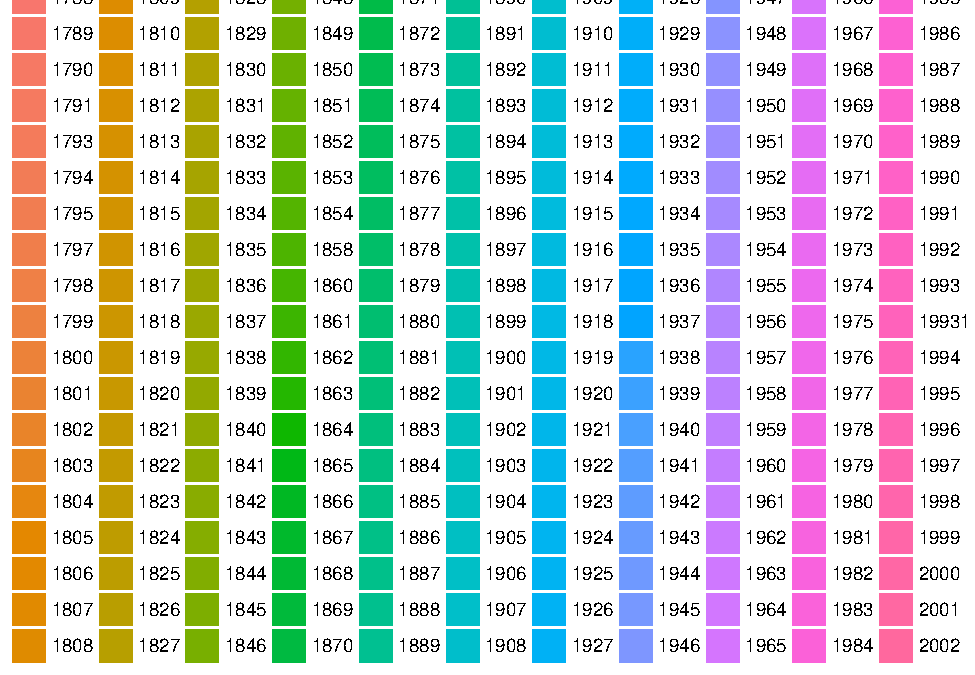
\includegraphics{JSturm-Proposal_files/figure-latex/analysis-one-1.pdf}

\subsection{Part 4: Inference}\label{part-4-inference}

\subsection{Conclusion}\label{conclusion}

\subsubsection{Relevant summary
statistics}\label{relevant-summary-statistics}

\begin{Shaded}
\begin{Highlighting}[]
\NormalTok{lvls <-}\StringTok{ }\KeywordTok{levels}\NormalTok{(amendments}\OperatorTok{$}\NormalTok{year)}

\KeywordTok{ggplot}\NormalTok{(amendments, }\KeywordTok{aes}\NormalTok{(year)) }\OperatorTok{+}
\StringTok{  }\KeywordTok{geom_bar}\NormalTok{() }\OperatorTok{+}
\StringTok{  }\KeywordTok{scale_x_discrete}\NormalTok{(}\DataTypeTok{breaks=}\KeywordTok{seq}\NormalTok{(}\DecValTok{1788}\NormalTok{, }\DecValTok{2014}\NormalTok{, }\DecValTok{20}\NormalTok{))}
\end{Highlighting}
\end{Shaded}

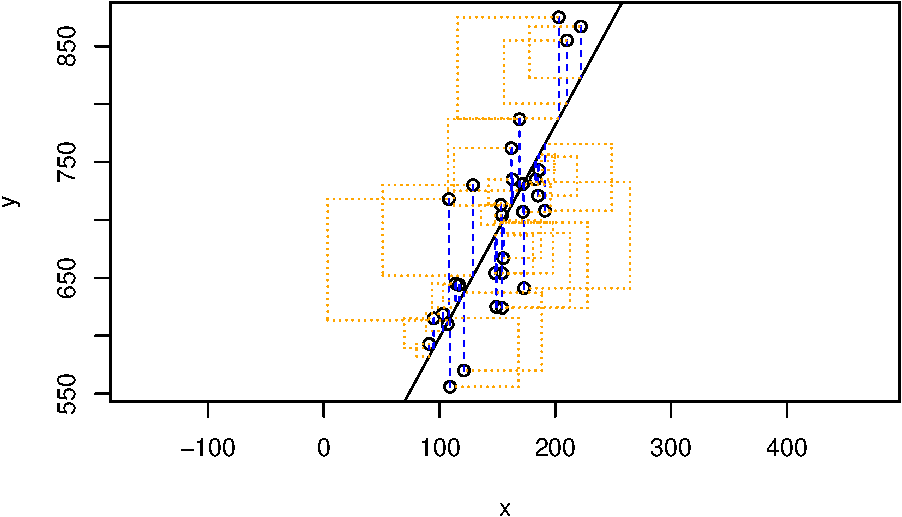
\includegraphics{JSturm-Proposal_files/figure-latex/unnamed-chunk-1-1.pdf}
There is a noticeable spike in amendmendt proposals in the latter half
of the 20th century. My guess would be that it's related to the civil
rights movement, and the sweeping changes that came about.


\end{document}
